%%%%%%%%%%%%%%%%%%%%%%%%%%%%%%%%%%%%%%%%%%%%%%%%%%%%%%%%%%%%%%%%%%%%%%%%%%%%%%
\section{Mu2e DAQ configuration}

\subsection{Configurations}

The system supports multiple configurations, as shown in Figure~\ref{figure:run_configurations}

\begin{figure}[H]
  \begin{tikzpicture}
    \node[anchor=south west,inner sep=0] at (0,0.) {
      % \node[shift={(0 cm,0.cm)},inner sep=0,rotate={90}] at (0,0) {}
      \makebox[\textwidth][c] {
        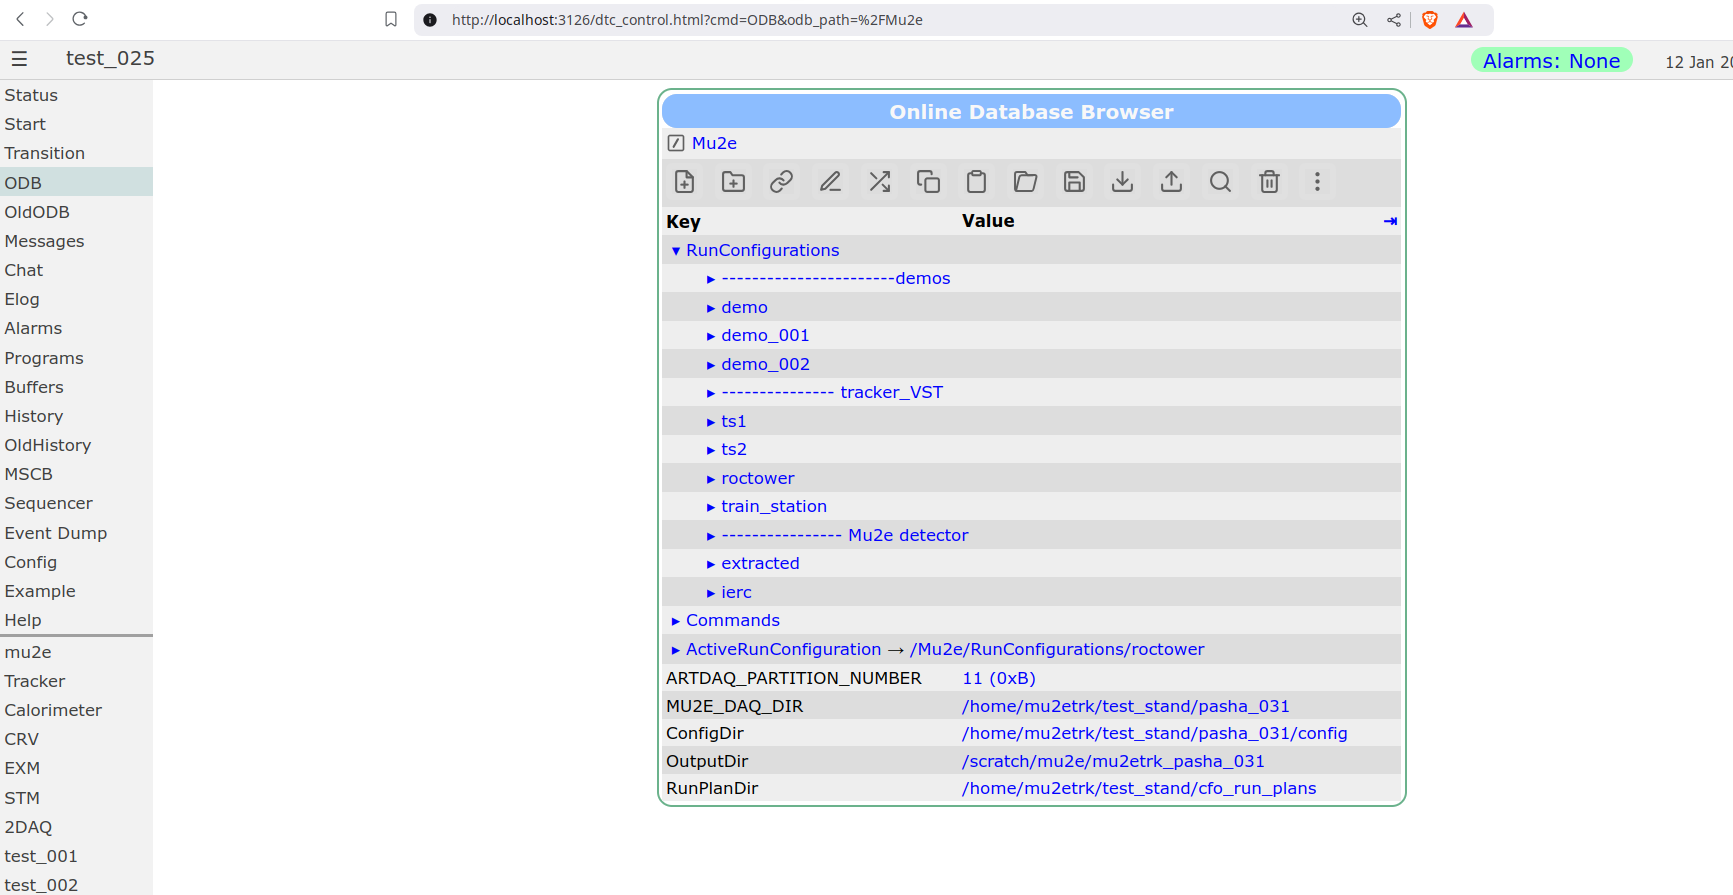
\includegraphics[width=0.95\textwidth]{png/run_configurations}
      }
    };
    % \node [text width=8cm, scale=1.0] at (14.5,0.5) {$\mu_B$, expected background mean};
    % \node [text width=8cm, scale=1.0, rotate={90}] at (1.5,7.5) { $S_{D}$, ``discovery'' signal strength  };
  \end{tikzpicture}
  \caption{
    \label{figure:run_configurations}
    Run configurations
  }
\end{figure}

Each configuration has a name, a status, and includes a set of subdetectors, as shown in

Figure~\ref{figure:configuration_top}

\begin{figure}[H]
  \begin{tikzpicture}
    \node[anchor=south west,inner sep=0] at (0,0.) {
      % \node[shift={(0 cm,0.cm)},inner sep=0,rotate={90}] at (0,0) {}
      \makebox[\textwidth][c] {
        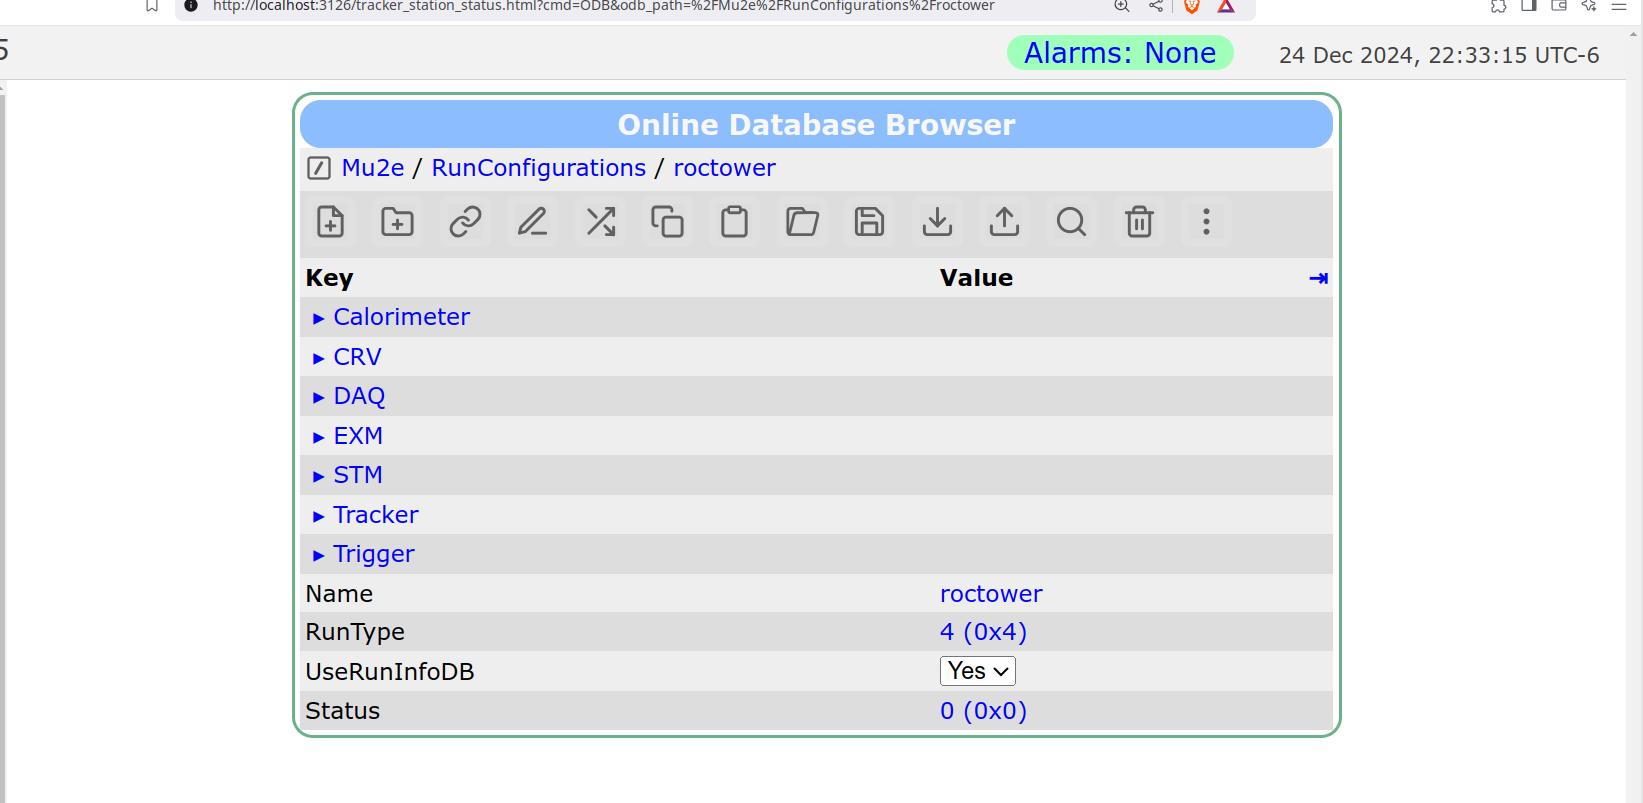
\includegraphics[width=0.95\textwidth]{png/configuration_top}
      }
    };
    % \node [text width=8cm, scale=1.0] at (14.5,0.5) {$\mu_B$, expected background mean};
    % \node [text width=8cm, scale=1.0, rotate={90}] at (1.5,7.5) { $S_{D}$, ``discovery'' signal strength  };
  \end{tikzpicture}
  \caption{
    \label{figure:configuration_top}
    Top view of the configuration called 'roctower' - a 6-ROC tracker test stand in IERC
  }
\end{figure}

Each element has two fields, ``Enabled'' and ``Status'', used for monitoring - see
Figure~\ref{figure:tracker_config}

\begin{figure}[H]
  \begin{tikzpicture}
    \node[anchor=south west,inner sep=0] at (0,0.) {
      % \node[shift={(0 cm,0.cm)},inner sep=0,rotate={90}] at (0,0) {}
      \makebox[\textwidth][c] {
        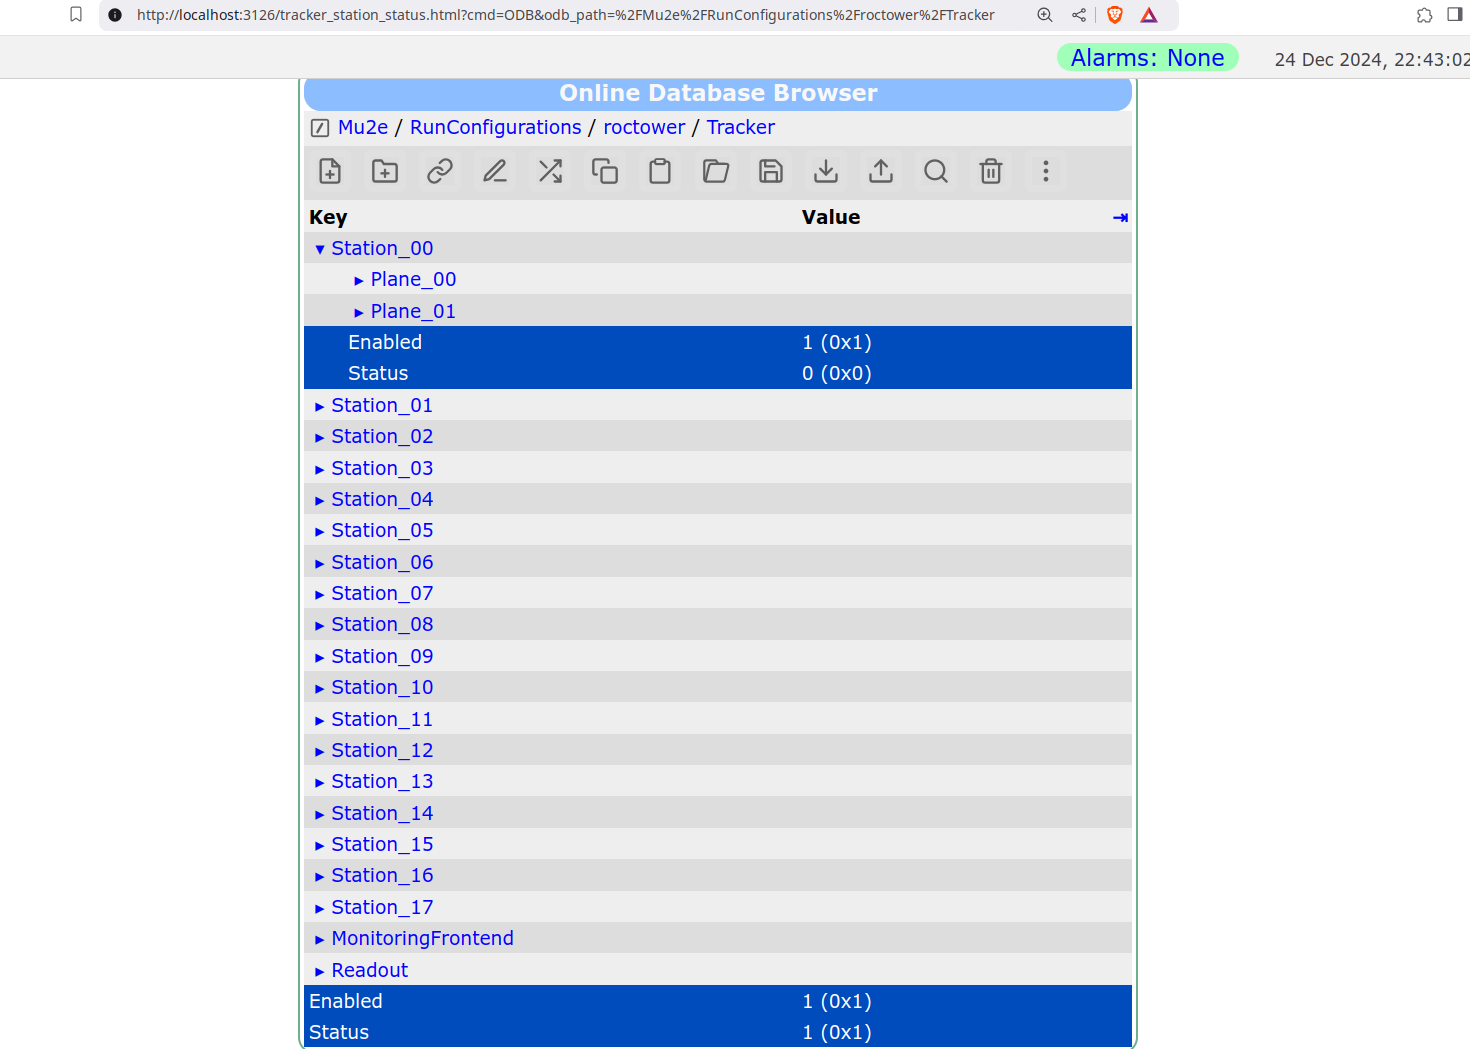
\includegraphics[width=0.95\textwidth]{png/tracker_config}
      }
    };
    % \node [text width=8cm, scale=1.0] at (14.5,0.5) {$\mu_B$, expected background mean};
    % \node [text width=8cm, scale=1.0, rotate={90}] at (1.5,7.5) { $S_{D}$, ``discovery'' signal strength  };
  \end{tikzpicture}
  \caption{
    \label{figure:tracker_config}
    Tracker configuration. The tracker, as well as each of the stations, has ``Enabled'' and
    ``Status'' fields.
  }
\end{figure}



\subsection{Data Model}

* configuration  : first step                                                
- request run number
- set "CONFIGURE" in /Mu2e/Commands/ (this could be done via the Sequencer)

- a configuration frontend (python)
  - identifies enabled subdetectors
  - passses the command to the enabled subdetector configuration frontends (python)
  - the subsystem configuration frontends are completely independent
  - waits for some time for them to act
  - subssytem configuration frontends complete, set Status and 
  - after the configuration succeeds or the time expires, the configuration
    frontend forces stop of its execution
  - it sets the command execution status and returns to MIDAS

- if the configuration step has completed successfully, a new run is started

- each subsystem has Enabled and Status attributed in ODB
- to exclude the failed sysbystem from the configuration: set Enabled=0

- DAQ configuration:

  - CFO configuration
  - configuration of each node

  - per node:

    - one or two boardreaders
    - event builder
    - data logger
    - dispatcher

    - each of them has Enabled attribute

  - TFM talks to ODB , identifies enabled processes and submits jobs only
    for them

  - there is a "Generate FCL" command which generates FCLs
    for an given? active? configuration

- as the DAQ configuration depends on the enabled detector configuration,
  the DAQ is configured afer all subdetectors 


* monitoring of the detector status                                          

- each subdetector has "Enabled" and "Status" parameters
\begin{verbatim}
|--------+-----------+--------------------------------------------|
| status | color     | meaning                                    |
|--------+-----------+--------------------------------------------|
|     -2 | dark gray | Enabled=0                                  |
|     -1 | gray      | enabled=1, but no initialization performed |
|      0 | red       | enabled=1, failed initialization           |
|      1 | green     | enabled=1, initialized OK                  |
|--------+-----------+--------------------------------------------|
\end{verbatim}

* description in ODB                                                         
- no links across configuration boundaries
- links allowed within the configuration , i.e.
  - DTC --> tracker panel
  - boardreader DTC --> DTC configuration
- ActiveConfiguration
* commands and execution
 a command has three fields
 
1) Run     : 0: "no request to run"  1: "requested to run" 
2) Status  : int
   < 0: "execution failed" , the value gives the error code
   0  : "execution finished OK"
   1  : "execution in progress"

   after the Status is set, the same client resets Run=0
3) Parameters :


%%%%%%%%%%%%%%%%%%%%%%%%%%%%%%%%%%%%%%%%%%%%%%%%%%%%%%%%%%%%%%%%%%%%%%%%%%%%%%
\subsection{Configuration of the frontends}

\begin{itemize}
\item
  one monitoring/control frontend per DAQ server . MOnitoring:
  \begin{itemize}
  \item
    2 DTC's with 6 ROCs per DTC
  \item
    ARTDAQ processes:
    \begin{itemize}
    \item
      2 boardreaders, N event builders, potentially a data logger, and a dispatcher
    \end{itemize}
  \item
    overall health: amount of free space available
  \end{itemize}
\item
  global control frontend:
\end{itemize}
%%% Local Variables:
%%% mode: latex
%%% TeX-master: t
%%% End:
